\chapter{Software System}
\label{chap:softwareSystem}

The online visualization toolkit is implemented as an additional tool for accessing plant data on Energy-Charts. Energy-Charts is build using JavaScript libraries. Therefore, same, or corresponding technologies were used for our interactive visualization map. 

The vision of this project is to provide an interactive map for users who are interested in Germany’s electricity production.  This visualization tool provides multiple possibilities to explore the Germany’s electricity generation and its distribution. First, users can get an overview of power plants. It shows the location, operating status, and generation capacity of all renewable and conventional power plants in Germany. Second, this interactive map is associated with ThemeRiver or stacked area charts where users can see an hourly production of electricity for each power plant. Finally, the tool also visualizes the power transmission lines (110kV, 220kV, and 380kV) of Germany. Furthermore, users can select multiple power plants and list them in a table chart for comparison. It is also possible to compare those selected units and based on their hourly production with Energy-Charts. 

\section{Requirement Analysis}
\label{sec:reqAn}

As mentioned before, to implement Energy Chart JavaScript library is used. Plant data are stored as JSON files on the server. Hence, for creating an interactive map as an extension to the Energy Chart and to match the functionality with the existing charts, JavaScript mapping library is also used for this project. Our goal was to create an interactive map which is dedicated to the power plants of Germany. Before implementing the tool, the basic must-have components for the map must be specified. Therefore, following things were considered as a list of requirements for the map to enable a quick exchange of information between users and the map.

\section*{System Requirements}
\begin{itemize}
	\item{Need to develop an interactive map with OpenStreetMap open source JavaScript libraries.}
	\item{For having no data base, our tool must be able to access JSON files from the server using AJAX query and deliver it to the map.}
	\item{The interactive map should run on web platform, support web technologies and usable on modern smart devices.}
\end{itemize}

\section*{Interface Requirements}
\begin{itemize}
	\item{To visualize the location of the plants, glyph based visualization technique can be used. A meaningful map marker must be used for each fuel source category. A fixed color code is assigned to each source category.}
	\item{In the case of mouseover or clicking event a marker, window, or tool-tip must appear displaying the basic information of the power plants. Displayed information needs to be extracted from given JSON files.}
	\item{In addition, the high voltage power lines should be displayed on the map for three voltages 110kV, 220kV, and 380kV.}
	\item{To complete the interface, a simple, clean, and effective navigation menu must be designed and should be placed above the map to display or hide different types of power plants and high voltage power lines.}
\end{itemize}

\section*{Functional Requirements}

\begin{itemize}
	\item{Internal communication between the interactive map and Energy-Charts must be established. Thus, the users can query plant data, see their hourly production, and can make a comparison.}
	\item{The map and energy charts have to be linked. Therefore every selection is reflected in both and that people should be able to chose individual power plants.}
	%\item{A way of comparison between power plants must be established.}
	\item{Navigation menu and its utility  should offer adequate possibility to allow user for controlling the view on the map API}
\end{itemize}

Therefore, to achieve and implement the above-mentioned requirements we decided to use a simple lightweight JavaScript mapping library – Leaflet.  Finally, we end up with a fully-clickable interactive map as a composite image consisting of a map, location markers and poly lines. 

In the following, we will give an overview of the architecture and explain the graphical user interface of the visualization tool.

\section{Architecture}
\label{sec:architecture}

The diagram in Figure \ref{fig:architecture} shows the architecture of the complete interactive map and its connection between server-side and client-side. 

Back-end is developed based on JavaScript along with the Leaflet. Additionally, jQuery and underscorejs are used to eliminate the necessity to reprogram the basic operation and functionality. Multimedia contents and JSON files are loaded on the FTP server. 

Initially, leaflet and additional JavaScript code for creating the map API are executed on the page load. By default, JavaScript code makes request to the file server over HTTP and get JSON files as a response. Location of all power plants are preserved in that JSON file. Leaflet parses the JSON file and render the power plants on the map. During this operation program also set the marker properties. Each source category has a unique marker image which are also stored in the server. At the end users get an interactive interface and can see the map on the screen with some colorful markers of power plants locating its location on the map. 

There is an individual script that executes after page load for establishing the connection between front-end and back-end. All the JavaScript events for navigation menu, buttons and map zoom-in/out events are registered there. The large GeoJSON files for high voltage power lines are not initially loaded. User needs to use the navigation menu for sending a new HTTP request to see them on the map. Server identifies the path of the requested file through scripts and returns the GeoJSON file to the client side. Finally leaflet parses the GeoJSON data and render it to the map.


\begin{figure}
  \begin{center}
    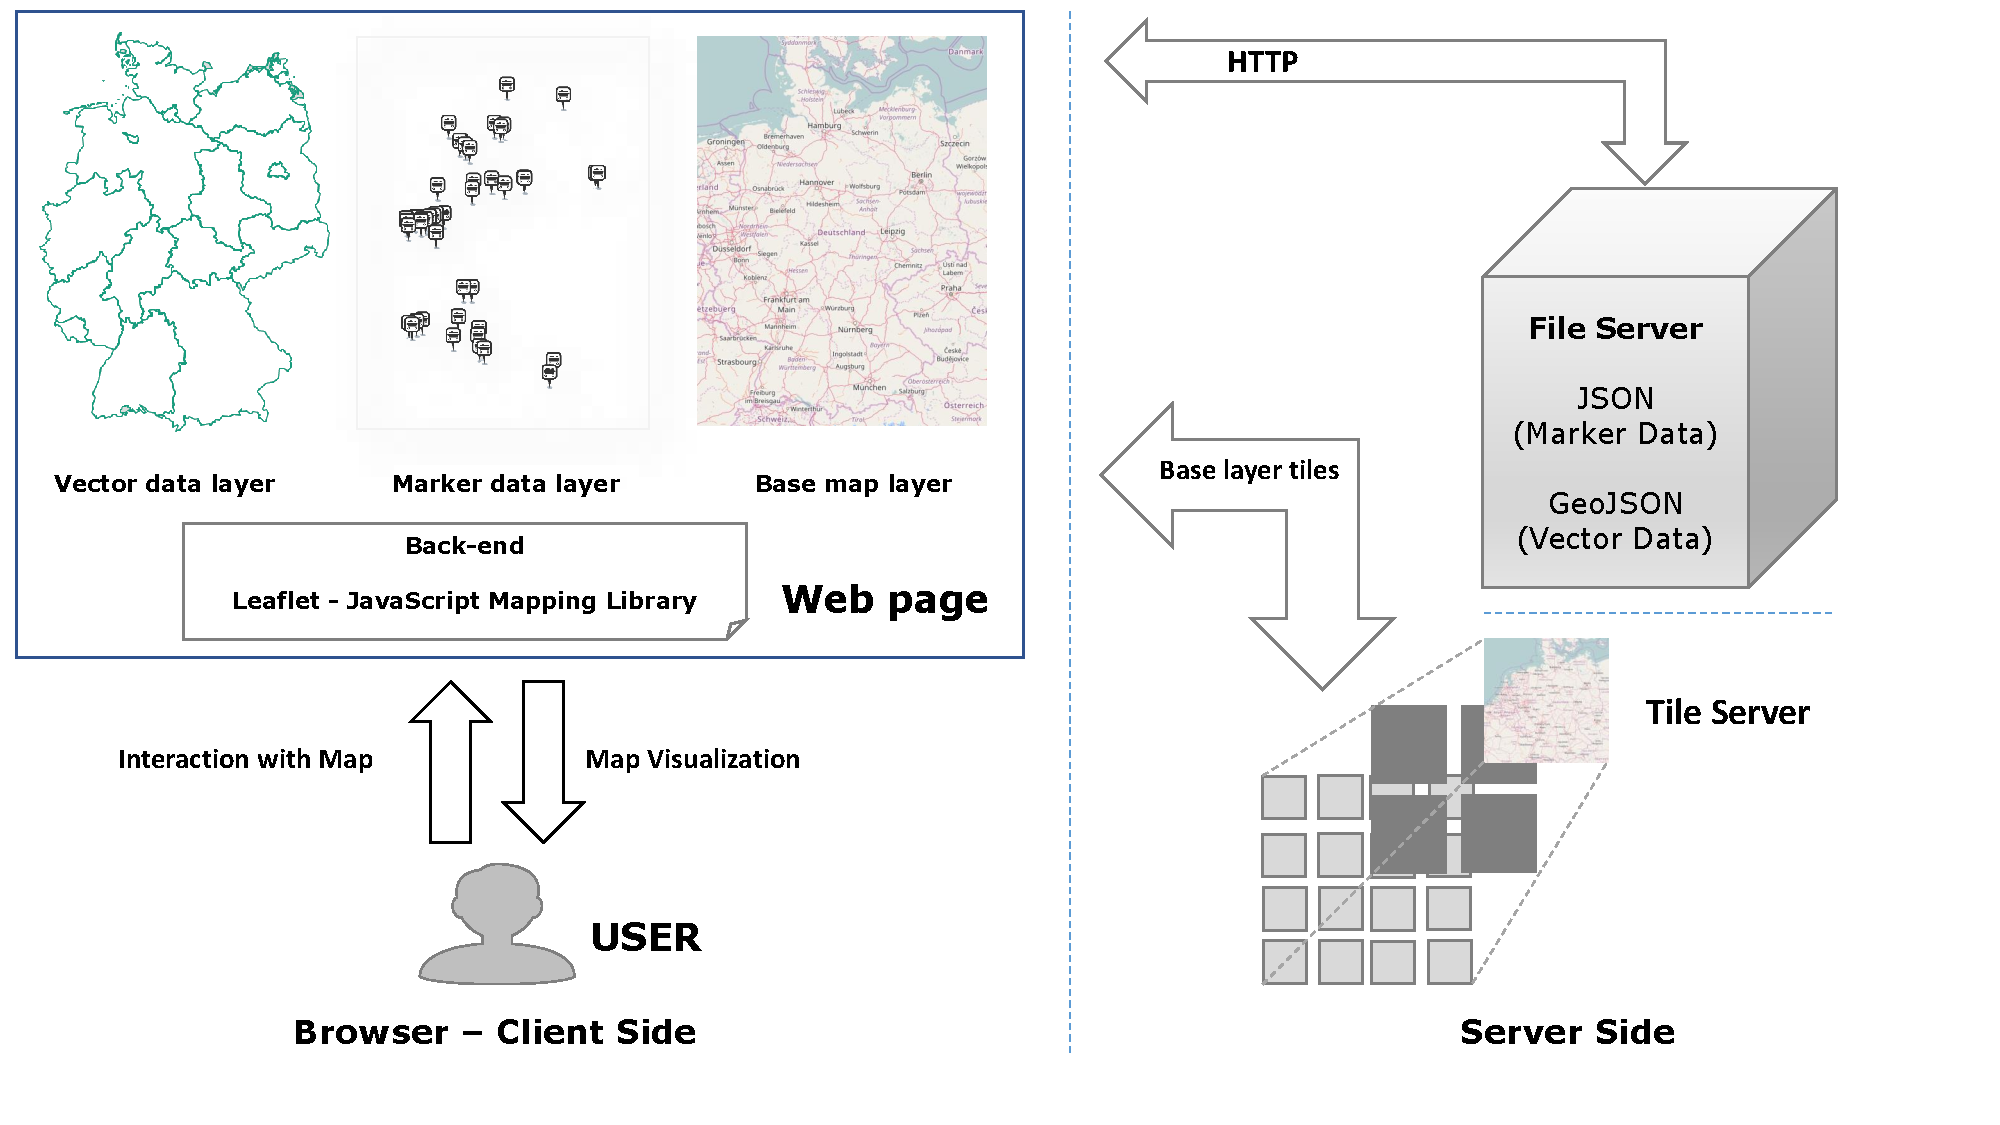
\includegraphics[width=1\textwidth]{architectureNew}
    \caption[The architecture of the visualization tool]{The architecture of the visualization tool - connection between back end and front end}
    \label{fig:architecture}
  \end{center}
\end{figure} 

\section{User Interface}
\label{sec:ui}

Based on the back-end the front-end is entirely developed in HTML, CSS, and JavaScript using the existing template for Energy Charts. Bootstrap design system was chosen for interface(e.g navigation menu, buttons and drop down) design and making the web page responsive. Furthermore, the user interface of interactive map is designed for desktop computers as well as smart mobile devices. In the following, the main structure of the graphical user interface containing the navigation menu, map API as well as the comparison chart will be presented. The main structure is shown in the Figure \ref{fig:structure}. As this interactive map is integrated into the Energy-Charts page, therefore the same template is used for the header section. Our graphical UI starts right after the navigation menu of the Energy-Charts page. Our interactive visualization tool starts with a navigation menu which can also be called as a control layer for the map. Check-boxes are used for the navigation menu area to externally control the map. They are decorated with unique colors. These colors are matched with the colors that have been assigned to each source category in the JSON file.  The map is located under the control layer where markers, power lines, and their basic information are displayed. An area for comparison list is allocated on the web page. Comparison table chart only appears when a user selects a power plant for comparison. Depending on the device, the appearance of the comparison list may change. Hence, our online interactive data mapping tool consists of three main parts: 

\begin{itemize}
	\item{Control Layer: Navigation menu with two subsections}
	\item{Map API: Cluster layer, markers, high voltage power lines, legends and basic information in the pop-up box}
	\item{Comparison List: Comparison table chart for comparing power generation of the power plants that fall under same source category.}
\end{itemize}

\begin{figure}
  \begin{center}
    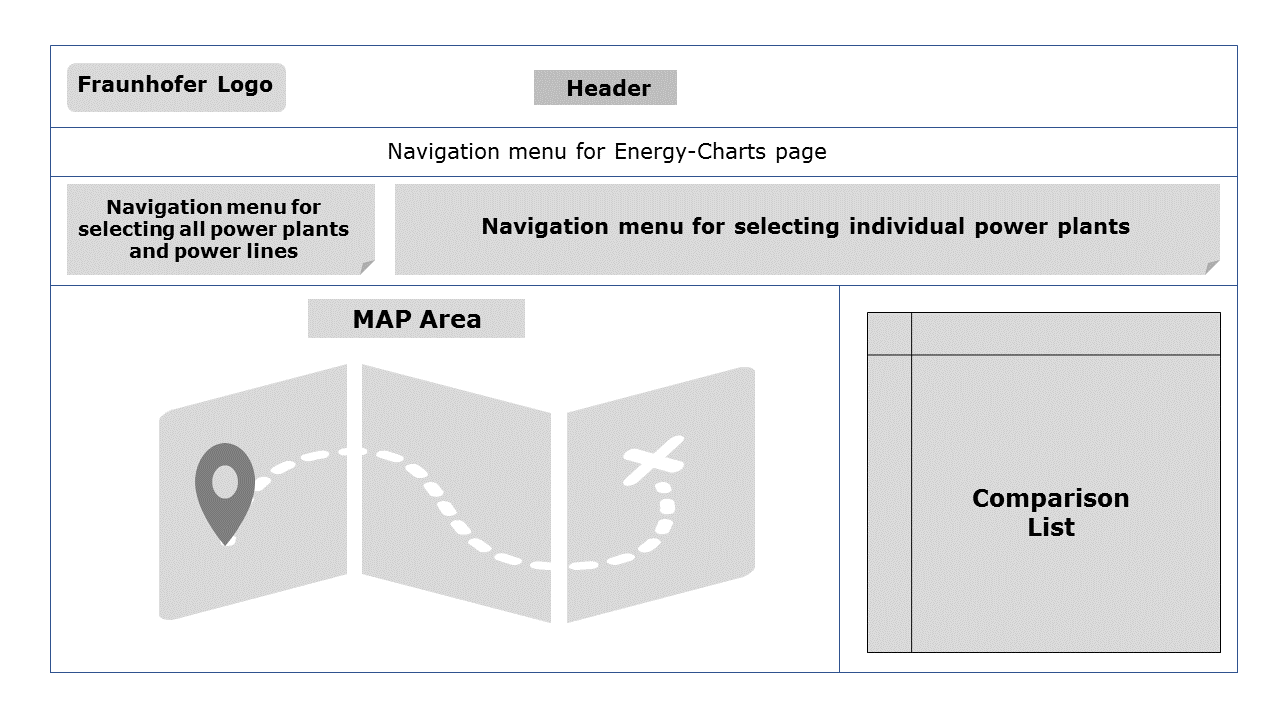
\includegraphics[width=1\textwidth]{structure}
    \caption{The main structure of the visualization page}
    \label{fig:structure}
  \end{center}
\end{figure}

In the following these parts are particularized in details.

\subsection{Control layer}
\label{sssec:controlLayer}

Control layer provides the functionality to manage the displayed content on the map. Check-boxes are used to control the map using external JavaScript events. It is possible to design these boxes in different ways. This circular design is inspired by the legends of energy power chart. For this reason, we designed this external navigation menu for controlling the map. Control layer is divided into two sections (See Figure \ref{fig:menuu}).

\begin{figure} [H]
  \begin{center}
    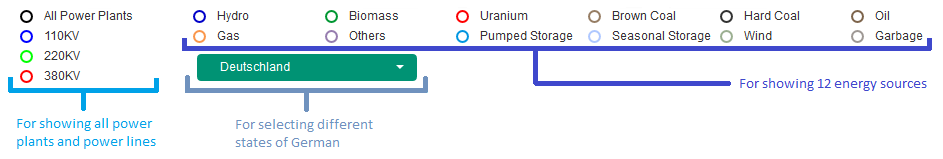
\includegraphics[width=1\textwidth]{menu}
    \caption{Navigation menu}
    \label{fig:menuu}
  \end{center}
\end{figure}


Check-boxes for selecting all power plants at once, and for high voltage power lines are located on the left side of the navigation menu. In the remaining space, check-boxes for selecting individual energy sources category are placed on the right side of the navigation menu. As provided in the JSON data, there are 12 energy source categories are provided in the navigation menu. Check-boxes are decorated with a circle with a border and a label next to the circle. A tool tip appears under it if the user hovers the mouse over the check-box (see Figure \ref{fig:menuTT}. Check-box area includes the circular check-box and its label. 

\begin{figure} [H]
  \begin{center}
    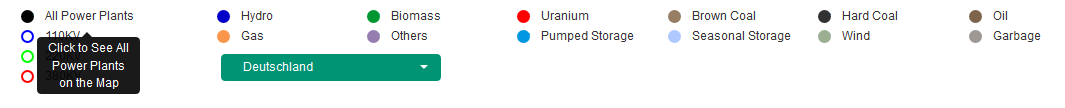
\includegraphics[width=1\textwidth]{menu_tooltip}
    \caption{Tool tip for Check-boxes}
    \label{fig:menuTT}
  \end{center}
\end{figure}

A drop-down selection menu is designed to locate and select 16 different states of Germany on the map. %sIt can be used to select between 16 German states in the form. It contains a header and labels for each state. 


\subsubsection*{Control Layer Properties}

Control layer is an essential part of the interactive map. To perform an action, the user needs to select check-boxes. When the status of the check-box is not selected or unchecked, its appears as an empty white circle with a colored border. On selection, it is filled with its previously assigned border color (see Figure \ref{fig:menufilled}) and reveals the power plant on the map. For example, to show all power plant on the map the user must click on the check-box labeled with “All Power Plants”. This action triggers all 12 check-boxes of power plants and fills the circles with colors (see Figure \ref{fig:menu2}). While continuing this operation if any one of the power plants is unchecked or deselected, then “All Power Plants” is automatically deselected.  On the other hand, if all 12 check-boxes are selected manually, this action also selects the check-box of “All Power Plants”. Therefore, based on selection the content of the map will be updated. Same properties and behaviors are also applicable for individual high voltage power lines. To see the power lines on the map, the user must select the check-boxes assigned for each power line. 

\begin{figure} [H]
  \begin{center}
    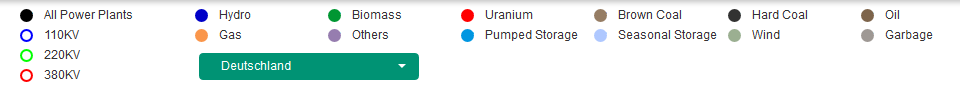
\includegraphics[width=1\textwidth]{menu_filled}
    \caption{Navigation menu with all power plant selected.}
    \label{fig:menufilled}
  \end{center}
\end{figure}

\begin{figure} [H]
  \begin{center}
    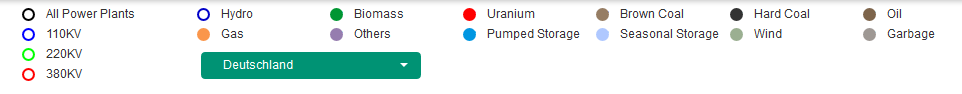
\includegraphics[width=1\textwidth]{menu_one_not_selected}
    \caption{Navigation menu where one energy-source is deselected.}
    \label{fig:menu2}
  \end{center}
\end{figure}

The drop-down selection mechanism for German states is also a part of the control layer. It was added to give users an opportunity to control the map and find different states inside Germany. Users can choose between 16 states from the menu for zooming in and to have the local view of that particular state. This animated zoom-in option uses a feature of Leaflet to get the bounds of the selected state data layer and fits on the map with the maximum possible zoom level. This will help the user to get an idea about the power plant density inside the selected state of Germany. The user needs to select “Deutschland” to restore the global view of the German map. Figure \ref{fig:stateSelection} shows an example of state selection mechanism. On the selection of Baden-Württemberg from the drop-down list, it is highlighted, and map zoomed in to fit it on the map screen.

\begin{figure}
  \begin{center}
    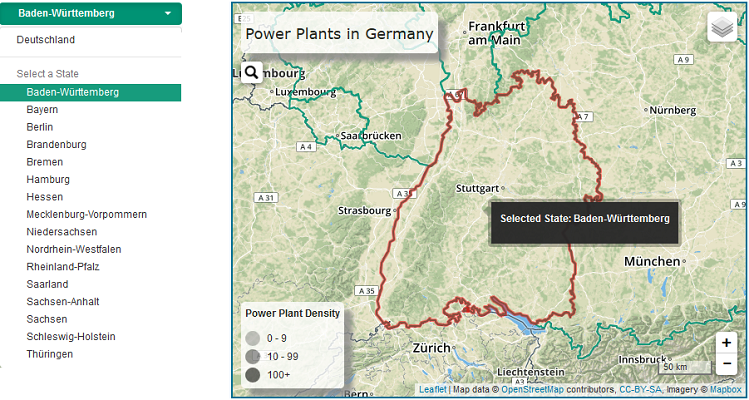
\includegraphics[width=1\textwidth]{state_selection}
    \caption[A German state (Baden-Württemberg) is highlighted]{A German state (Baden-Württemberg) is highlighted, when it is selected from the drop-down navigation menu}
    \label{fig:stateSelection}
  \end{center}
\end{figure}

\begin{figure}
  \begin{center}
    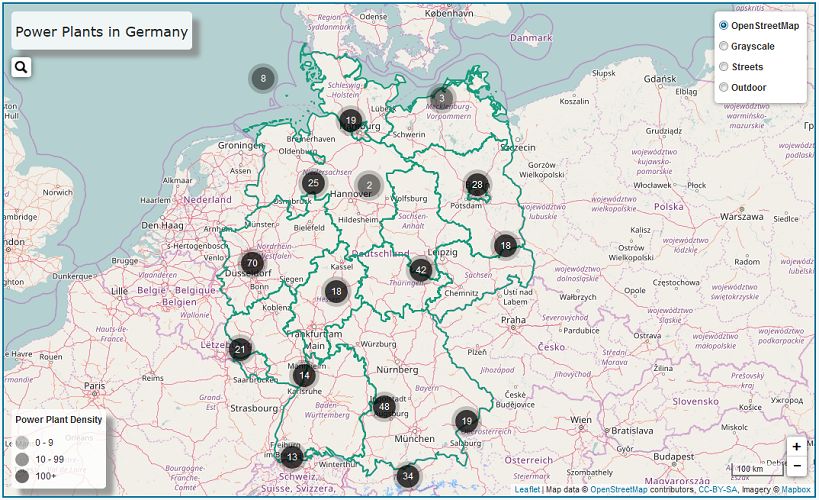
\includegraphics[width=1\textwidth]{map_view}
    \caption[Interactive map area]{Interactive map area equipped with legends on (top-left and bottom-left), initial cluster view, zooming and map scale control (bottom-right), different base map layer controller(top-right)}
    \label{fig:mapView}
  \end{center}
\end{figure}

\subsection{Map API}
\label{sssec:mapArea}

The interactive map appears under the navigation menu on the web page. Our initial view of the map, when the page opens, is illustrated in Figure \ref{fig:mapView}. After initializing the map, the default view of the map is set to Germany with a zoom level 6. Therefore, the entire map of Germany is visible in the map area. The area is equipped with legends, zoom controller, and map scale controller. The custom control layer is collapsed and placed on the top-right corner of the map. Beside these, another information layer is added by default to highlight the border of Germany and its states. This vector data layer is a collection of polygons and stored as GeoJSON on the server. This GeoJSON was extracted from GitHub\footnote{Databundeslander, \url{https://gist.github.com/oscar6echo/4423770} (last accessed on \today)}. In addition, a cluster view of all markers was created using Leaflet.MarkerCluster plugin and was added to the map. This cluster view could help the user to understand the density of power plants of a particular area. The number written inside of a cluster represents the total number of markers contained under this. Cluster layer is filled with black color and its opacity depends on the density of the markers. A custom control legend is added to the bottom-left corner of the map area describing the color scale. When user mouse over a cluster it shows the bound of its markers and if the user clicks on a cluster it zooms to its bounds. As discussed in Chapter~\ref{chap:background} Section~\ref{sec:clusterr}, this plugin is also helpful to find if there are more than one plant located at the same position on the map.

\subsubsection{Functionality}
\label{sssec:functionality}

\begin{figure} [H]
  \begin{center}
    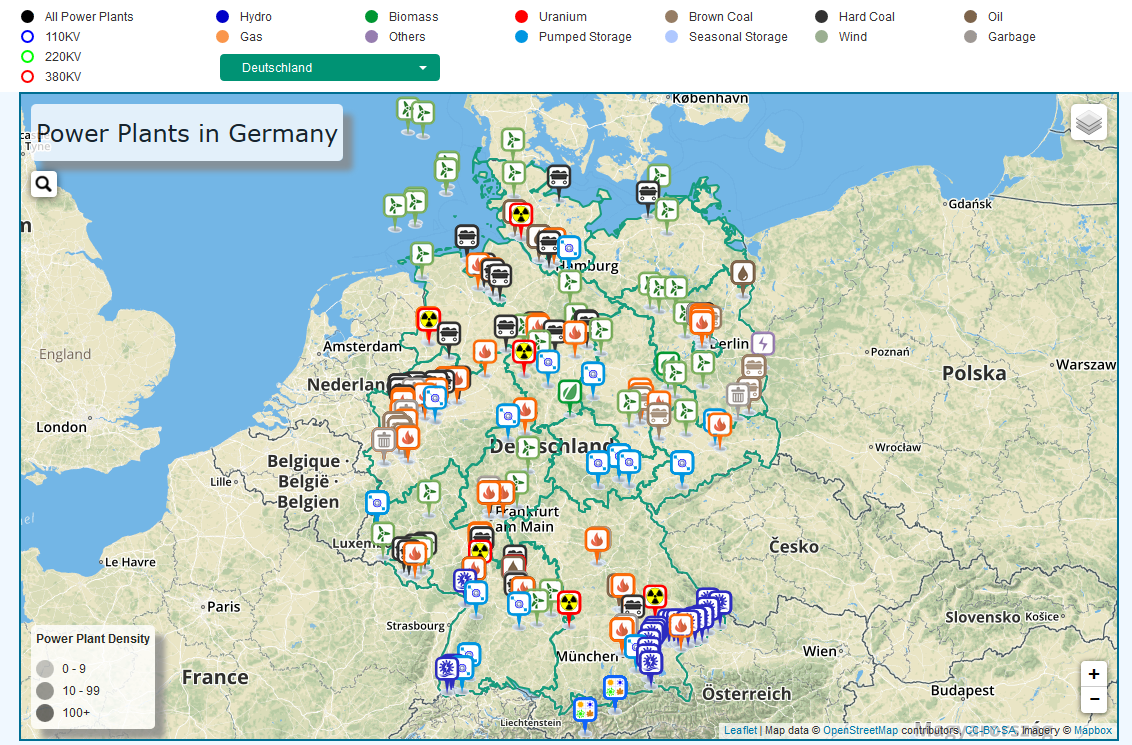
\includegraphics[width=1\textwidth]{marker_ini}
    \caption{Showing the geographical location of all power plants with markers.}
    \label{fig:markerini}
  \end{center}
\end{figure}

In this section, the functional aspects of our visualization tool in the combination with our control layer are discussed.

As discussed in Section \ref{sssec:mapArea}, by default a cluster view of all power plants are rendered on the map. This is added as a layer on the map. Cluster view interprets that there are no check-box selected or no action was performed externally on the map. From this position, users can zoom in by clicking the zoom-in button or even by scrolling the mouse. Markers smoothly split from the cluster on zoom-in and merge to its cluster on zoom-out. If any check-box is selected, this action will remove the cluster layer from the map. In the case of viewing all power plants on the map, the user needs to select “All Power Plant” and as a result, all the markers are visible on the map (see Figure \ref{fig:markerini}). For Each energy source category, a unique color and marker logo are assigned. At the time of reading the JSON data, markers are categorized and stored in groups. Each object of layer group is rendered on the map as a check-box input. For example,  to see all nuclear power plants, the user needs to select the check-box labeled “Uranium”. In that case, only the nuclear marker layer object is added to the map (See Figure \ref{fig:uranium}. Here, jQuery is used for targeting the html DOM (Data Object Model) input check-box object and leaflet functionality is used to add it to the map. 

\begin{figure}
  \begin{center}
    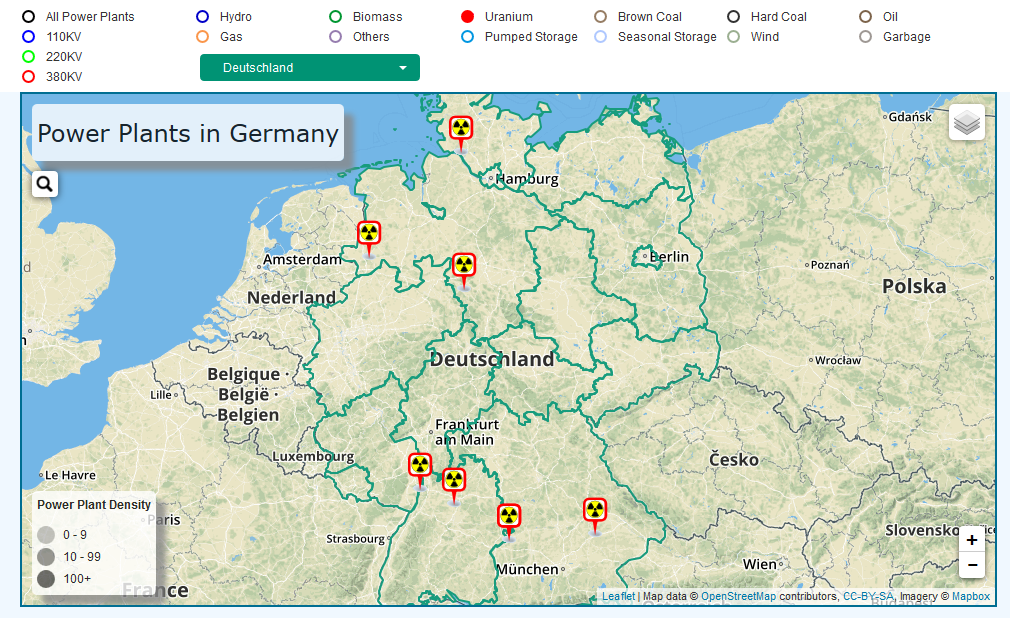
\includegraphics[width=1\textwidth]{uranium_selected}
    \caption{Showing all nuclear power plants.}
    \label{fig:uranium}
  \end{center}
\end{figure}

Along with the geographical location representation, information about each power plants have also been attached to its location marker. Every time a user clicks on a marker a pop-up is attached to it with a specified HTML content and finally, the pop-up appears on the center of the map. We have used a custom design for the pop-up. It is a table with details on the power plant, two buttons, and colored border. Figure \ref{fig:mpp} shows two different pop-up boxes for two different power plant categories. It is clearly visible that they are similar in structure but not in color. The color of the border and the button varies for different categories. This pop-up box is used for displaying the basic information of power plants from the JSON. Basic information includes unit name,unit id, source, capacity, company name, start date and some other additional information. 


\begin{figure}
  \begin{center}
\subfloat[A marker pop-up of Gas power plant\label{fig:gaspp}]
  {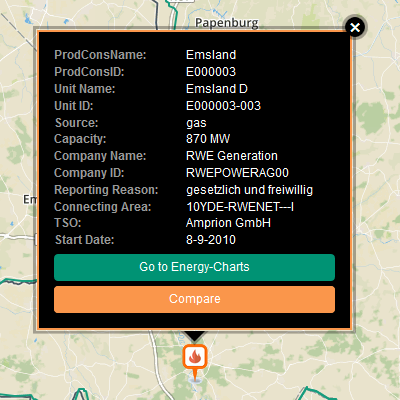
\includegraphics[width=.45\linewidth]{gas_pop}}\hfill
\subfloat[A marker pop-up of Nuclear power plant\label{fig:npp}]
  {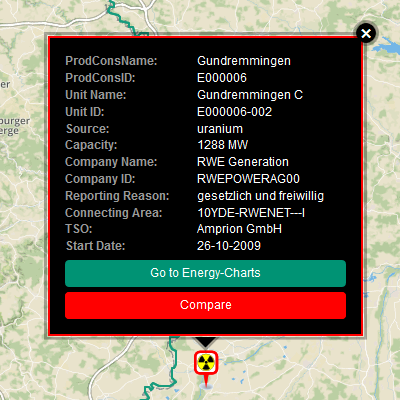
\includegraphics[width=.45\linewidth]{uranium_pop}}
\hfill
\caption{Marker Pop-up box}
\label{fig:mpp}
\end{center}
\end{figure}

\subsubsection{Connectivity between map and energy-charts}
\label{sssec:connectivity}

In this section, the connectivity between interactive map and energy chart is discussed. This was one of the main functional requirements for our interactive map application.

Our goal was to access and view the hourly electricity production data of each power plant from the interactive map. Therefore, an internal connection is established. Users can select power plants and send a query to the energy charts to see their production. If the data of that specific power plant unit is available on the server, then hourly production of that power plant will be illustrated on energy charts. Users are informed over a browser pop-up window on the energy chart page if there is not data available.

The interactive map provides two possibilities to access power plant data on the energy charts. First approach, using the “Go to Energy-Charts” button, which acts as a link (see Figure \ref{fig:buttons}.  Users can send a query by clicking on the “Go to Energy-Charts” button to directly view the time line visualization of electricity production. Each of this button has a unique link for sending queries. These links are dynamically generated while inserting the basic information of power plants in the pop-up box. This link delivers information to the chart. These information are \textit{source} and \textit{ID}. Each power plant has a unique unit id and source category, which are provided inside the power plant JSON data as an object. The hourly production JSON data also have the same object for unit id but its source category is specified inside the file name. Therefore, the value of \textit{source} variable is required to query the desired file and the value of \textit{ID} is required to match the desired power plant data. Hence, only one power plant production data is visible on the hourly production chart and others visibility are hidden. Second approach is using the "Compare" button, which leads to the Comparison List. Comparison list and its application for accessing electricity production data is discussed in the Section \ref{sssec:comparisonList}.

\begin{figure}
\centering
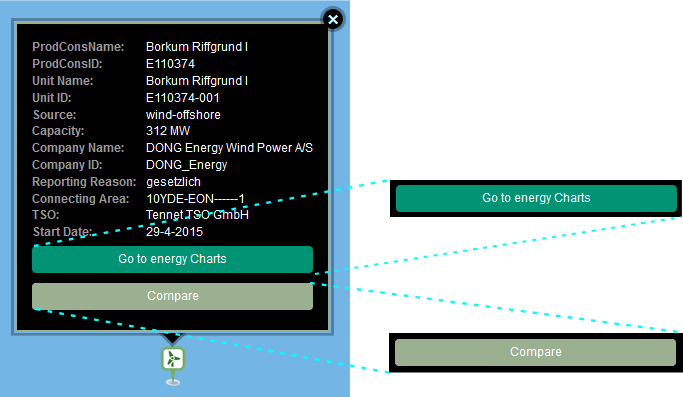
\includegraphics[width=1\textwidth]{buton}
\caption[Buttons inside pop-up box]{\textit{Go to energy charts} button - to see its electricity production on energy chart and \textit{Compare} button - to add this plant to the comparison list}
\label{fig:buttons}
\end{figure}

\subsection{Comparison List}
\label{sssec:comparisonList}

Our interactive map provides an additional feature, where users can compare multiple power plant, and in the end, users can view their hourly electricity generation on the chart. A click on the “Compare” button (see Figure \ref{fig:buttons}) generates a comparison list (see Figure \ref{fig:ctable}) on the interactive map page. The comparison list will appear next to the map (or below, for mobile devices). Users can dynamically add more power plants to the list. Newly added plants are listed as a new entry on the table. If a plant is added to the table then its “Compare” button is disabled and marked as “Selected”. This function prohibits adding the same element several times to the list. The hourly production data of the power plants in the comparison list can also be shown in the Energy Charts by clicking the “Compare on Energy Charts”. This describes the second of approach for accessing hourly electricity generation data. Like “Go to Energy-Charts” button, “Compare on Energy-Charts button also acts as a link. This new button also passes information upon clicking it. Unlike the first approach, this link passes the information from the comparison table. Therefore, more than one power plant data is visible on the charts. Figure \ref{fig:eccharts} shows the hourly production data for the wind-offshore power plants because only those three power plants are listed in the comparison table. This function runs when users click on the "Compare on Energy Charts" button. 

\begin{figure} [H]
\centering
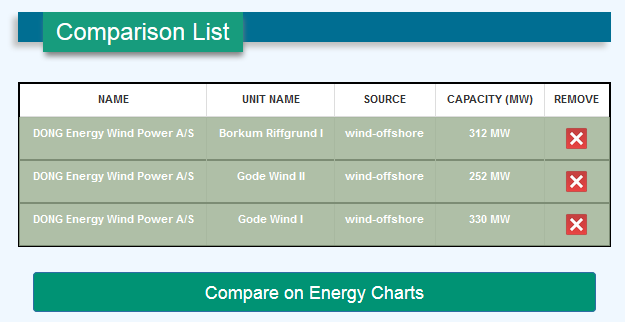
\includegraphics[width=1\textwidth]{comparison_table_wind}
\caption[Wind-offshore(3) power plants are listed on the comparison table]{Wind-offshore(3) power plants are listed on the comparison table. Table also includes a button (\textit{Compare on Energy Charts}) to see their hourly production on energy chart.}
\label{fig:ctable}
\end{figure}

\begin{figure}
\centering
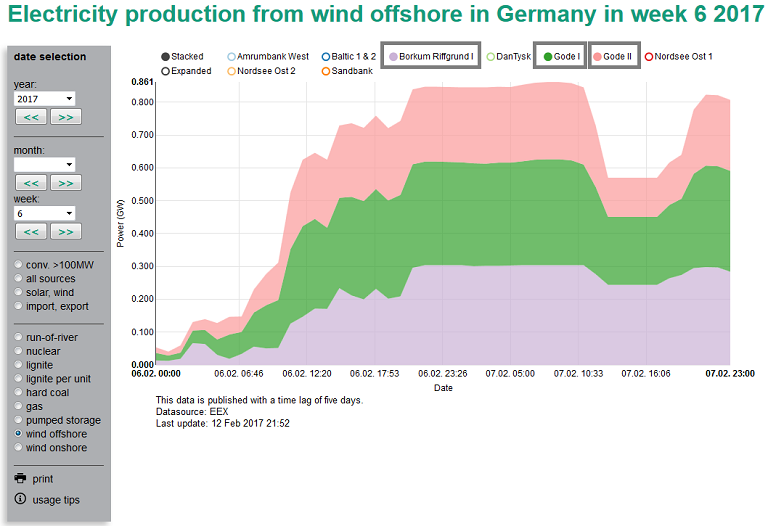
\includegraphics[width=1\textwidth]{ecchart}
\caption[Energy Chart showing the hourly production data]{The chart is created after clicking the "Compare on Energy charts" button in Figure \ref{fig:ctable}. Wind-offshore is selected in the left navigation area (source) and only listed power plants are selected and the rest are deselected.}
\label{fig:eccharts}
\end{figure}

Only power plants from the same source category can be compared on the comparison list. Users can add as many power plants as needed in the comparison list from different source category but this approach disables the functionality to compare them on energy charts page. For example, if users are interested to view the electricity production of Nuclear(Uranium) power plants then users should include only Nuclear power plants to the comparison list and use the "Compare on Energy Charts" to see their production. Currently, the energy charts can only illustrate the hourly data for a single source category. There is a form, inside the gray area with some radio buttons, for controlling the chart and to see the electricity production on the chart for different sources (see Figure \ref{fig:eccharts}). Energy charts provides the unit wise electricity production data for Hydro, Nuclear, Brown Coal (lignite), Hard Coal, Gas, Pumped storage, Oil, Wind-offshore, and Wind-onshore power sources. At present there is no data available for Biomass, Seasonal storage, Garbage, and Others source category. Therefore, it is not possible to see their production and compare them on energy charts.   

\section{Data query process on energy charts}
\label{sec:algorithm}

In the Section \ref{sssec:connectivity}, how the interactive map is connected to the energy charts is already discussed. The algorithm used for solving this functional requirement is separated from that discussion and described here in details. 

As mentioned before there are two different ways to access and view the hourly electricity production data. The basic difference between these two approaches is not much. “Go to Energy Charts” button passes only two variables (\textit{source} and \textit{ID}) over URL and direct to energy chart page. Figure \ref{fig:url} shows how the underlying link of the button is updated dynamically. 

\begin{figure} [H]
\centering
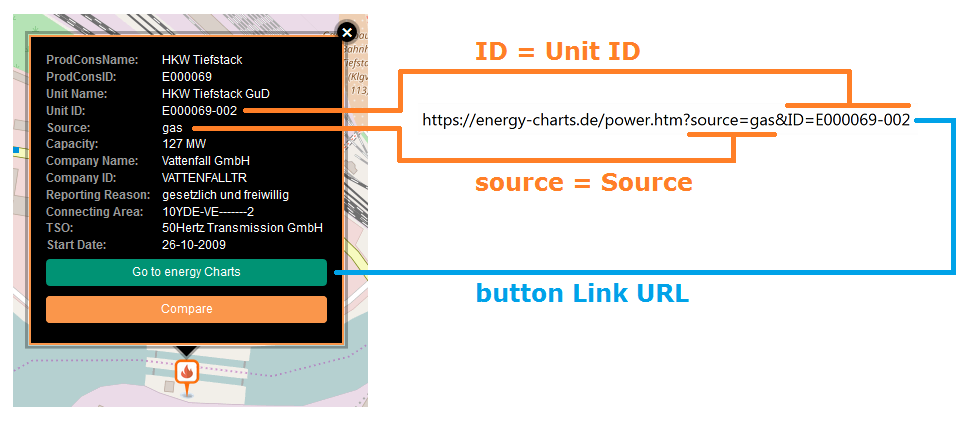
\includegraphics[width=1\textwidth]{url}
\caption{Hyperlink of "Go to Energy Charts"}
\label{fig:url}
\end{figure}

The functionality of "Compare on Energy Charts" button is also discussed before in Section \ref{sssec:connectivity}. The functionality of this button is to pass one or more unit ids over the URL. When a user adds a new power plant to the comparison list, the unit id of that power plant is added inside the \textit{ID} variable. Consequently, the link of the "Compare on Energy Charts" button is updated in the background. Figure \ref{fig:stepsPP} shows different steps of adding more than one power plant in the comparison list and how the link is updated in every step. This approach starts when users want to compare one or more than one power plants. For example, a user wants to compare the capacity and hourly production of three Nuclear power plants. In Step 1, user opened a pop-up window of a Nuclear plant and added this to the comparison list by clicking on the "Compare" button. Step 2 and Step 3 can be done in the similar way. Therefore, two more power plants are added to the comparison table. Thus, in total three unit ids are added to the \textit{ID} and the redirect link for "Compare on Energy Charts" is updated as showed in the Figure \ref{fig:stepsPP}. 

\begin{figure} [H]
\centering
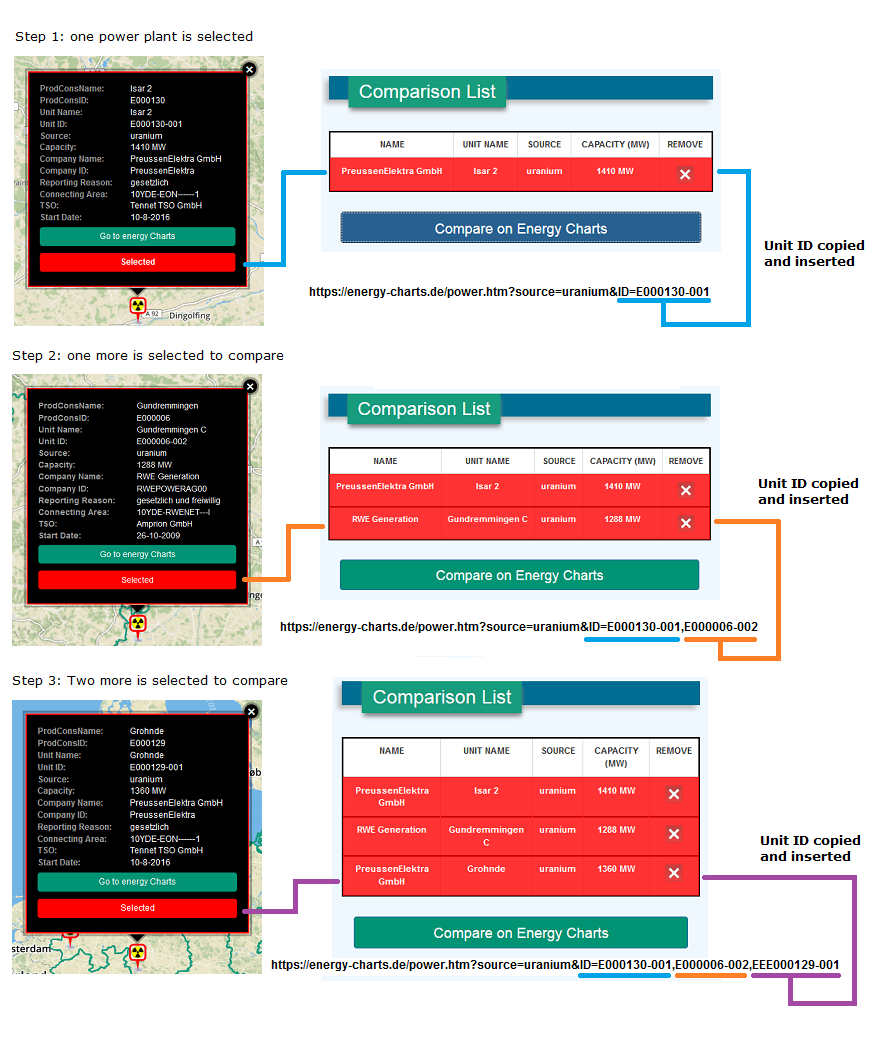
\includegraphics[width=1\textwidth]{multiplechart}
\caption[Steps of adding power plants to the comparison list]{Step 1: a nuclear plant is added into the comparison list - unit id added to the link; Step 2: another nuclear plant is added - new unit id added; Step 3: The last one is added into the list - unit id added and link is updated}
\label{fig:stepsPP}
\end{figure}

Electricity production data are all stored in JSON files. Charts always load the data dynamically and plot these files according to user selection. Every JSON file name is written in several parts. It has a unique source name, week and year. The week and year is manually set when the data for that particular week is available on the server. On having URL variables, energy chart uses these and creates the chart accordingly. URL variables are handled by JavaScript and stored it locally for further operation. “source” variable is used to select the radio button of that particular source category on the navigation menu and also to complete the filepath (see List \ref{lst:url-json}). Radio button initializes the filepath using the source name. List \ref{lst:url-json} shows an instance of the first step of handling URL variables. This operation is similar for both approaches. 

%[language=json,firstnumber=1]
\begin{Listing}
\begin{lstlisting}
var _unitID = []; // Empty array for storing ID from the link 
var _sourceName = getUrlVariables()["source"]; // Variable for storing the source name from the URL variables

_unitID = getUrlVariables()["ID"]; // get the ID/IDs from the link an stores inside this array

if (_sourceName != undefined && _unitID != undefined) { // checks if source and id are available inside the url

	var defaultradiob = "disp_"+ _new_sourceName; // Selects the radio button for selecting source

	var filepath = "./power_unit/week_"+ _path_source_name +"_"+ defaultyear +"_0"+ defaultweek +".json"; //file on first-load using link variables
}

\end{lstlisting}
\caption{URL variables are handled using JavaScript}
\label{lst:url-json}
\end{Listing}

\begin{figure}
\centering
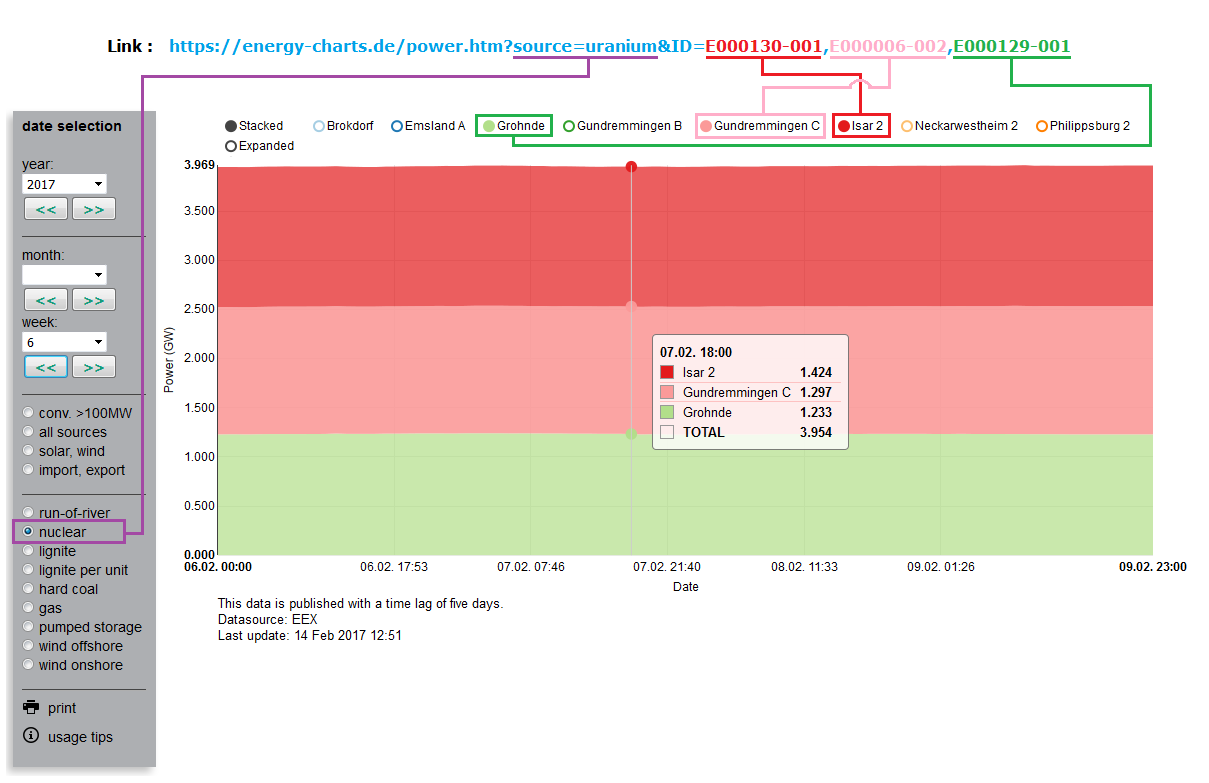
\includegraphics[width=1\textwidth]{ecselection}
\caption{Selected power plant data from the comparison table of Figure \ref{fig:stepsPP}}
\label{fig:ecselect}
\end{figure}

In the next step, algorithm handles unit ids from the URL. "Go to Energy Charts" link passes only a single unit id and "Compare on Energy Charts" link passes and array of unit ids. Figure \ref{fig:stepsPP} shows the impact of URL parameters to the electricity production chart. Source name from URL activates the radio button from the chart control area and unit ids are used to enable the visibility of those power plants on the chart. Therefore, circular legends are filled with colors. Other available power plant data is hidden from the chart thus circular legends are transparent. If there is no data available for selected units in JSON, then chart will load its default view instead. Default view of this chart enables the visibility of all power plants on the chart. 

%[language=javascript,firstnumber=1]
%\begin{Listing} [H]
%\begin{lstlisting}
%
%//Function for creating chart
%createChart(_sourceName, _unitID);
%
%function createChart(_sourceName, _unitID){
%	
%	// _sourceName is used for activating the radio button
%	_disp_source_unit = document.getElementById('radio button id').checked;  
%	
%	// _unitID is required here
%	if (_unitID != null) { // checks if unit ids is available on the URL
%		var uni_id = _unit_ID;
%		var query_list = []
%		query_list = uni_id.split(","); // array of unit ids - if more than one unit ids available //separate them using coma.
%	}
%	
%	// Function is ready for operation
%}
%
%\end{lstlisting}
%\caption{Function for creating chart with user defined parameter}
%\label{lst:createChart}
%\end{Listing}

NVD3\footnote{Official NVD3 Website, \url{https://nvd3.org/} (last accessed on \today)} JavaScript library has been used for creating chart on Energy-Charts page. It is a widely used charting library which is written in d3.js\footnote{Official D3 Website, \url{https://d3js.org/} (last accessed on \today)}. An instance of hourly production data file is shown in the List \ref{lst:dataFile}. This input JSON array has four attributes but only \textit{eexUnitID} is required to fulfill our requirements. The \textit{eexUnitID} of the hourly electricity production data and the unit id of the power plant location data (see Figure \ref{fig:stepsPP} are both the same ids. Our algorithm checks whether this eexUnitID exists inside the array of \textit{query list} or not. If exists then it is rendered on the chart. %List \ref{lst:algo} showing the JavaScript code for checking the URL parameter from the input data series.

%[language=JSON,firstnumber=1]
\begin{Listing} [H]
\begin{lstlisting}
// example of 
var inputData = [
{	"key": [{ "en":"Name_en" , "de":"Name_de" , "fr":"Name_fr" , "it":"Name_it" }] ,
	"color" : "rgb(number,number,number)" ,
	"eexUnitID" : "E000###-00#",
"KwNrBNetzA" : "BNA####" ,
	"values" : [ [ 1485903600000 , 0 ] , [ 1485907200000 , 0 ], [........]]}
]

\end{lstlisting}
\caption{Example of hourly production JSON data object}
\label{lst:dataFile}
\end{Listing}

[language=JSON,firstnumber=1]
\begin{Listing} [H]
\begin{lstlisting}
IF link variables exists THEN
   IF Only one eexUnitID exsits THEN
     loop1: REPEAT UNTIL < query list length
     loop2:  REPEAT UNTIL < eexUnitID length
					IF eexUnitID exist in query list
        	          enable series visibility 
                	  BREAK loop1
                	end IF
					ELSE Disable series
			 END loop2
		    END loop1
   end IF
   ELSE //for more than one eexUnitID
     REPEAT REPEAT UNTIL < query list length
       IF eexUnitID exist in query list
         Enable Series
         BREAK loop2
       end IF
       ELSE Disable series
     END for
end IF

ELSE Enable Series
\end{lstlisting}
\caption{JavaScript pseudo code for checking unit ids and enabling their visibility on the charts}
\label{lst:algo}
\end{Listing}

This part of the code is the new contribution to the existing energy chart. Line 1 of List \ref{lst:algo} checks the existence of parameter on URL. This function runs if URL parameters are available. Line 2 checks the number of the URL parameter (less or greater than 1). If the type of \textit{ID} is object then starts executing from line 2. Conversely, the function starts executing from line 13 if the number of \textit{ID} elements are more than one. Subsequently, function repeatedly checks the availability of unit ids from URL inside the data series. For this purpose, Line 6 enables the visibility of that data series on the chart if its unit id matches whereas unmatched data series are disabled on line 9. After executing this code users get the actual desired data illustrated on the chart which were queried over the link.

\section{Optimization of power line visualization}
\label{sec:powerLine}

In addition to the visualization of power plant location, showing the power transmission line is also a part of functional requirements. Therefore, our application provides an option for visualizing power transmission lines for 110kV, 220kV, and 380kV. Information about the data source is already discussed in Chapter~\ref{chap:background} Section \ref{sec:plsource}. Data was extracted in the format of geoJSON from the openstreetmap database. Figure \ref{fig:export} showing the available data formats that can be extracted using the overpass-turbo API. Leaflet supports GeoJSON and provides flexibility to map GeoJSON file there we have decided to use this format. Leaflet parses GeoJSON data and creates feature layers. Finally, the function displays the power transmission line to the map.

\begin{figure}
\centering
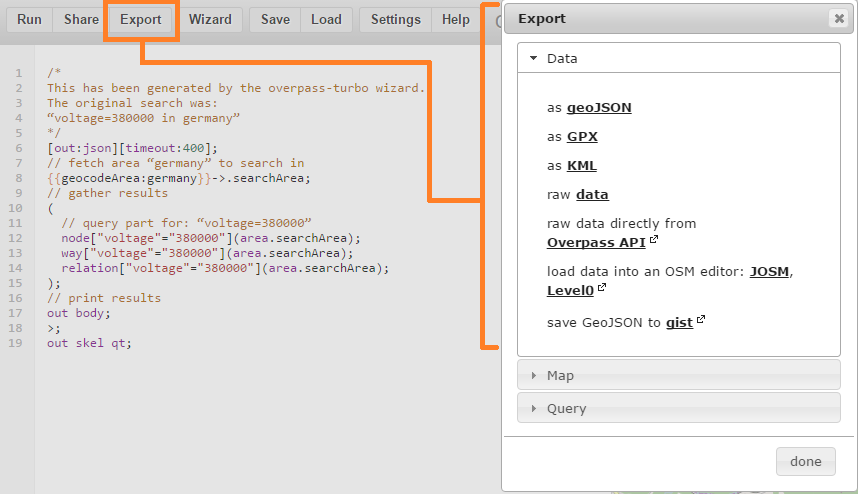
\includegraphics[width=1\textwidth]{export}
\caption{All possible data format that be extracted from the Overpass-turbo API}
\label{fig:export}
\end{figure}

The extracted GeoJSON data are too big in size. For the desktop computers it takes less than 2 seconds to load but Smart-phones and tablets take around 2 to 5 seconds for loading. Thus, it affects the performance of the map while zooming-in/out. Hence, it was required to optimize the process of mapping power lines. The following steps were taken to optimize the visualization of power lines.

\subsection{Map Bounds}

Leaflet provides extensive opportunities to control the map and provides current scale information about the map view. For our operation map bounds were considered for displaying the power transmission line on the map. It provides the lowest and highest value of latitude and longitude of the map view. Map bounds are changed every time the map is moved (either by zoom or pan).  Therefore, we used a function to reconsider the map bounds in every zoom level and display the GeoJSON data accordingly. Each time the map is moved, the map bounds is stored. If the power line data contains the map bound then the line is displayed otherwise it is skipped from mapping. Figure \ref{fig:mpbound} showing the power lines (380 kV) on 2 different zoom levels. In figure \ref{fig:mapBoundG}, map zoom level is 6 and whole Germany is visible inside the map bounds. Therefore, all the power lines data contains inside the current map bounds. Figure \ref{fig:mapBoundB} represents the map on zoom level 8 and showing the power lines that contains inside the current map bounds. Every time the map is moved, power lines are update according to the map bound. The Power lines which are outside the map bounds are skipped from operation. As a result, performance of the map was improved and loading time of the power lines were faster than before. List \ref{lst:plBound} showing the pseudo code for filtering the power line by utilizing the map bounds. Line 1 checks if the map has moved or zoomed-in/out and line 2 checks whether any power line is selected by users. A function for updating the power lines is called in line 4. Map update function is represented between line 8 to line 14 which is doing the filtering operation and return the layer to the map. 

\begin{figure}
  \begin{center}
\subfloat[Complete 380kV power line in the Germany (zoom level 6, no filtering)\label{fig:mapBoundG}]
  {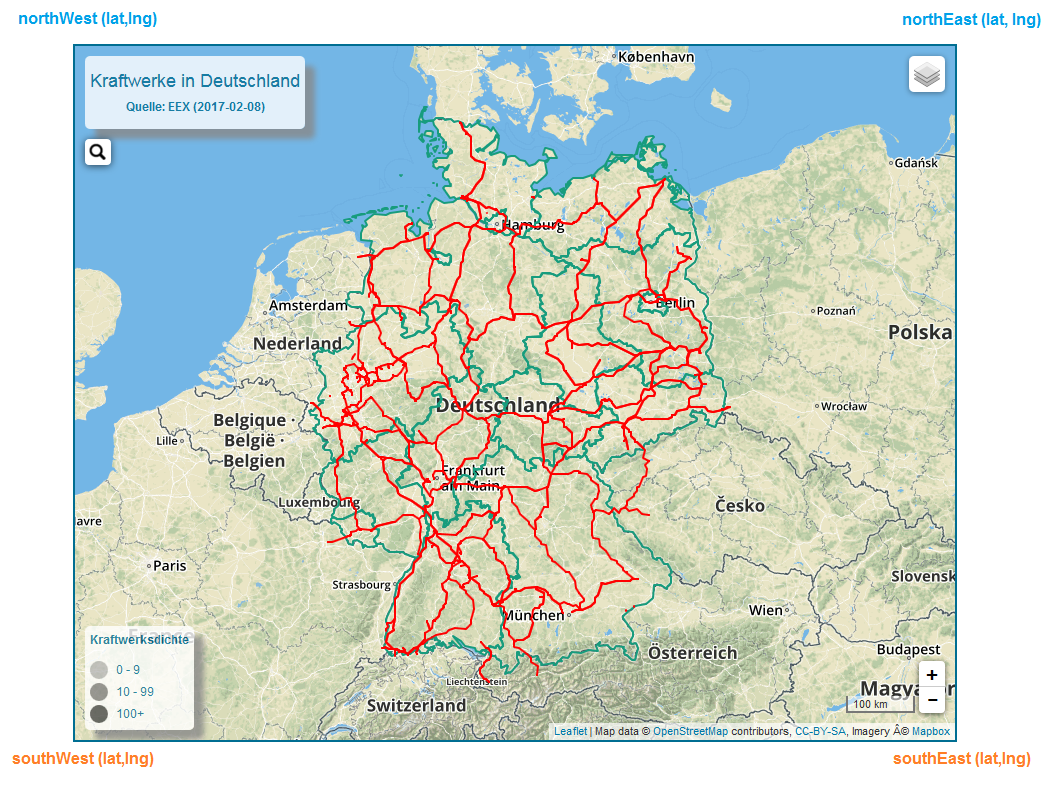
\includegraphics[width=.45\linewidth]{mapBoundGermany}}\hfill
\subfloat[380kv power line through Berlin (zoom level 8, filtered by map bounds)\label{fig:mapBoundB}]
  {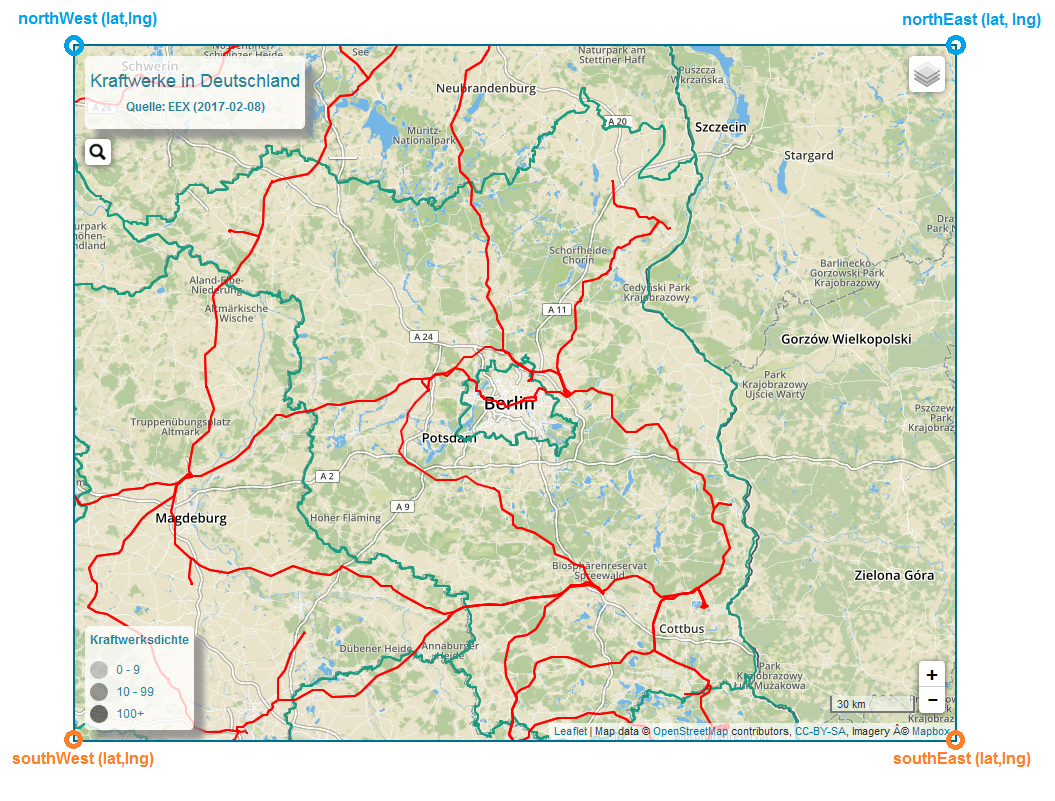
\includegraphics[width=.45\linewidth]{mapBound}}
\hfill
\caption{Filtering power lines depending on the map bounds}
\label{fig:mpbound}
\end{center}
\end{figure}

%[language=JavaScript,firstnumber=1]
\begin{Listing}
\begin{lstlisting}
ON map move ends or map zooming ends
	IF power line input selected
			DO remove previous layer
			CALL updateMap function
			DO add new power line layer
	end IF
// function for updating the map
FUNCTION updateMap
			GET map bounds
			CREATE power line layer
				IF layer contains map bounds
					ADD to layer
					RETURN layer
			end IF
\end{lstlisting}
\caption{Power line filtering algorithm depending on the map bound}
\label{lst:plBound}
\end{Listing}

\subsection{The Length of Power line}

The length of power transmission line is also considered for optimization. A long power transmission line is a collection of small sub layers of line string. These smaller line strings are affecting the performance of the map while loading.  For this purpose, smaller power lines are hidden on smaller zoom levels (when zoom level <= 8).  Small power lines contain a length between 1m to 500m. These smaller power lines are visible on higher zoom level ( zoom level > 8). This optimization is applied only for the 110kV power line. 110kV geoJSON data is relatively bigger in size and has more details than 220kV and 380kV transmission lines. 

This file has massive amount of entries for power lines and power stations. Polygons are describing mostly the power stations or substations inside the GeoJSON data and line-strings are describing the power transmission line. To visualize the proper routing and angle of power lines on the map, they are divided into many smaller parts inside the GeoJSON file. Our algorithm is hiding the power stations or substation, which are polygons, in smaller zoom level. Because, this smaller entries doesn't provide any useful feedback to the user. These smaller lines are available and added to the map on higher zoom level. Figure \ref{fig:plfilter} showing the power line density on different zoom levels. In figure \ref{fig:pl6}, power lines with smaller coordinate length (length > 45) are hidden where in figure \ref{fig:pl8} those lines have coordinate length less than 20 are hidden. The complete data information on 110 kV power lines are available when zoom level is higher than 9. Substations and smaller power transmission lines can be recognized at this zoom level. 

\begin{figure}
  \begin{center}
\subfloat[100kV power line (zoom level<6, coordinate length > 45)\label{fig:pl6}]
  {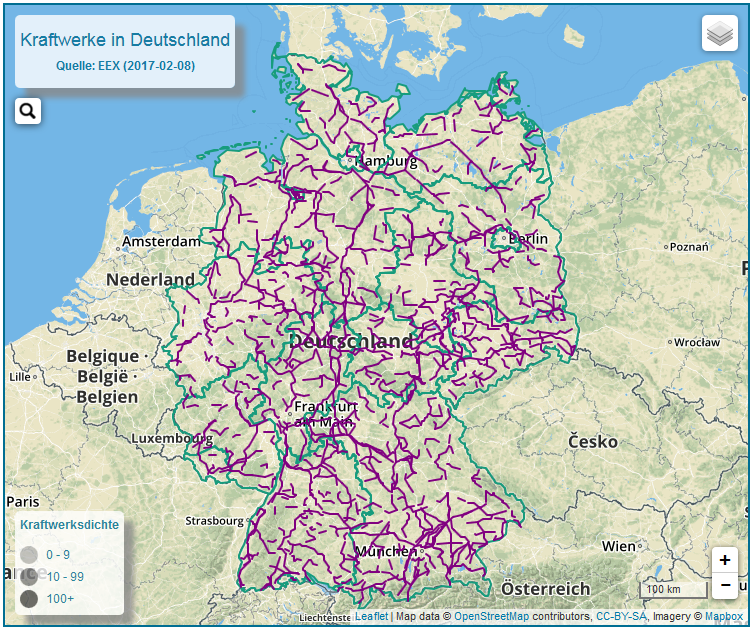
\includegraphics[width=.45\linewidth]{plzoom6}}\hfill
\subfloat[100kV power line (zoom level 8, coordinate length > 20)\label{fig:pl8}]
  {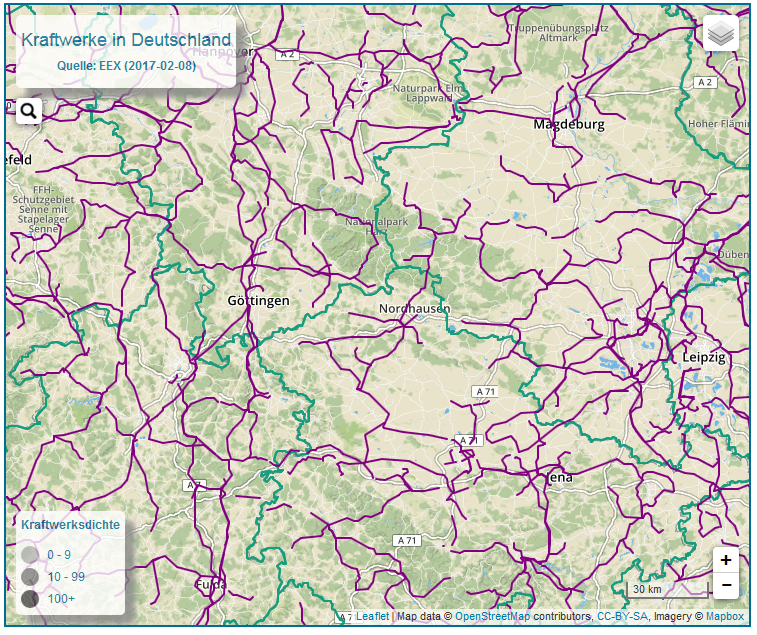
\includegraphics[width=.45\linewidth]{plzoom8}}
\hfill
\caption{Filtering power lines by coordinate length}
\label{fig:plfilter}
\end{center}
\end{figure}

\section{Summary and Discussion}

In this chapter, the implementation of the back-end and the front-end of the system was explained.
Furthermore, an overview of the graphical user interface as well as a detailed impression of
the architecture , interactivity scripting , interconnection process between map and chart was given. The visualization application solves the interface and functional requirements described in the Section \ref{sec:reqAn}. User are able to locate power plants and their hourly production data on energy chart. Furthermore, we assume that our visualization tool will help user to access the information of power plants as well as their hourly electricity production data. 
